\section{Einführung}
\todo{Vorlesung 20.9.21}

\subsection{Multiplexing}

\begin{enumerate}[nosep]
	\item Zeitmultiplex
	\item Frequenzmuliplex
	\item Codemultiplex
	\item Raummultiplex
\end{enumerate}

\subsection{Klassifizierung}
\begin{enumerate}[nosep]
	\item Energiesignal
	\item Leistungssignal
	\item Aperiodisch
	\item Periodisch
	\item Deterministisch
	\item Stochastisch
	\item Zeitkontinuerlich
	\item Zeitdiskret
	\item Amplitudenkontinuierlich
	\item Quantisiert
	\item Analog
	\item Digital
\end{enumerate}

\subsection{Kenngrössen} 
\todo{Vorlesung 27.9}

\todo{
	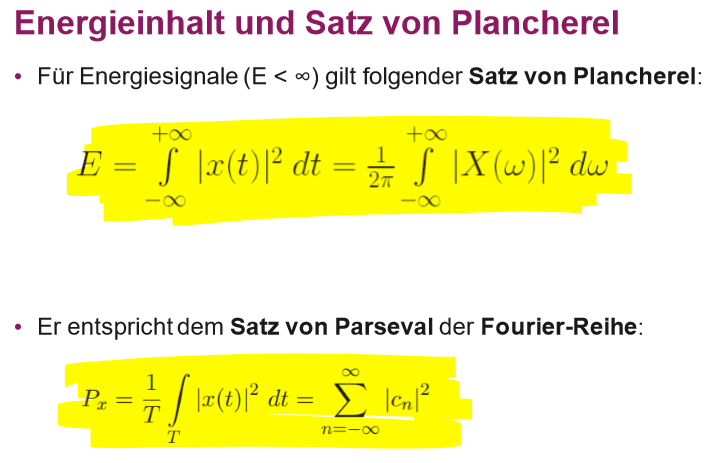
\includegraphics[width=0.7\columnwidth]{Images/screenshot002}
}

\noindent Momentanleistung: $P_x(t) = \left|x(t)\right|^2$\\
Mittlere Leistung: $\overline{P}_x =  \langle P_x(t) \rangle = \lim\limits_{T\rightarrow\infty}\frac{1}{T}\int\limits_{-T/2}^{+T/2}\left|x(t)\right|^2dt$ \\
Effektivwert: $x_{eff} = x_{rms} = \sqrt{\overline{P}_x}$ \\
Scheitelfaktor: $C = \frac{\max(\left|x(t)\right|)}{\sqrt{\overline{P}_x}}$

\subsection{Leistungsverhältnisse}
\todo{Übung 1.2 - Verstehen!}
[B] (Bel) ist ein $\log_{10}$ einer Leistung.\\
$k_{\text{P dB}} = 10 \log_{10}(\frac{P_y}{P_x}) \qquad [dB]$ \\

\textbf{ACHTUNG}: Bei Effektivwerten (RMS), da Eff. quadriert sind.\\ $k_{\text{P dB}} = 20 \log_{10}(\frac{y_{rms}}{x_{rms}}) \qquad [dB]$\\
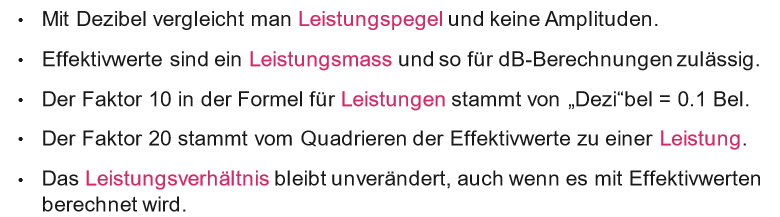
\includegraphics[width=\columnwidth]{Images/screenshot001}
